\documentclass[dvips,12pt]{article}
\usepackage[left=0.65in,top=0.3in,right=0.65in,bottom=0.3in]{geometry} % Document margins
\usepackage{paralist}
% Any percent sign marks a comment to the end of the line

% Every latex document starts with a documentclass declaration like this
% The option dvips allows for graphics, 12pt is the font size, and article
%   is the style

\usepackage[pdftex]{graphicx}
\usepackage{url}
\usepackage{amsmath}
% These are additional packages for "pdflatex", graphics, and to include
% hyperlinks inside a document.

\setlength{\oddsidemargin}{0.25in}
\setlength{\textwidth}{6.5in}
\setlength{\topmargin}{-0.5in}
\setlength{\textheight}{8.5in}

% These force using more of the margins that is the default style

\begin{document}
	
	% Everything after this becomes content
	% Replace the text between curly brackets with your own
	
	\title{Keyword Extraction by Deep Learning \\Mid Term Report}
	\author{Yi Cheng(yicheng1), Anoop Hallur(ahallur), Xiaoqiu Huang(xiaoqiuh)}
	\date{\today}
	
	% You can leave out "date" and it will be added automatically for today
	% You can change the "\today" date to any text you like
	
	\maketitle
	
	% This command causes the title to be created in the document
	
	\section{Introduction}
	
		As the goal of our project, we plan to do keyword extraction using deep learning. We are aiming to improve the performance of keyword extraction by deep learning techniques as compared to other techniques used previously.
		We believe that Deep learning techniques can improve the performance because when it has been applied to other similar tasks, a significant improvement has been observed.
		For example , Google speech recognizer uses Deep Neural Networks and accuracy is extremely high\cite{hinton2012deep}.The area of applying deep learning to keyword extraction has not been explored much, hence we are trying to apply it and see how it performs.
	\section{Related Work}
	
		Before diving into the details of our model and algorithm, we want to summarize the related work that has been done in the field of Keyword Extractions, how they can be applied to our project and how deep learning can be applied to solve this particular problem and our thoughts on why deep learning should give better performance compared to other algorithms.
		
		\subsection{Baseline Algorithms of Keyword extraction}
		
		A survey was done by Lott.B\cite{lott2012survey}, and he summarizes that whenever he have a large corpus of data already available(as in our case), TF-IDF is the most accurate algorithms of the existing ones. 
		
		In TF-IDF model, we assign weight to each term in the model, and we choose the top'n' weighted words as the keywords for the text. The weight of each word is computed by taking into account the Term Frequency(TF) and Inverse Domain Frequency(IDF), where Term Frequency indicates how significant is the term to a specific document, and IDF takes into account how common the word is in the domain. We have implemented the benchmarks for this algorithms on our dataset.
		
		The other algorithm proposed by Lott.B was the one using Lexical Chain approach. In this approach, the extract features from the document, first by constructing a lexical tree of the nouns in the document. They extract the nouns and each noun word is a possible tag for the document. The lexical chain is constructed using semantic features of the words such as other synonym, hyperonyms and morphynyms of a noun. From the lexical tree, they extract four features, and three features from other positional aspects of the nouns. The features are used to train a C4.5 decision tree and this decision tree is used to make predictions of the nouns in the document from the test data. We have implemented this particular algorithm for our data set and analyzed the results.
		
		Other algorithms presently being used are some variant of TF-IDF with domain specific modifications. For example , one technique uses a Bayes classifier with TF-IDF to compute the weights and extract the keywords. 
		There are techniques which are to be used when we don't have a corpus of text available to us. Frequency based single Document Keyword Extraction is one such technique. This techniques computes word weights by measuring the frequency of text occurrence within two punctuation marks in the text. Since we have text corpus available, we did not want to be compared against these classes of algorithms.
		\subsection{Deep Learning Intuition}
	\section{Model Description}
\subsection{Neural language model}
In traditional NLP model, the input of the classifier is just one-hot features or TF-IDF features of text. However, this model suffers from the curse of dimensionality. When the number of documents in the corpus becomes large, the matrix of features will become sparse. Therefore, Bengio et al.\cite{Bengio2003NLP} proposed a new neural language model which generates distributed representations for each word in the corpus. That means each word in the documents has a fixed length of feature vector. With the feature vectors of each term, we can measure the similarity between different words or generate the vector representation of each document.

In our model, each word will be first transformed to word vector by the tool named word2vec\cite{mikolov2013efficient}. The tool will first train the neural language model on our data set and then generate the word vector of each term.

\subsection{Recursive Autoencoder}
Autoencoder is a neural network model that learns the function $f(x)=x$ in order to learn the reduced representation of the input text. As we can see in the figure 1, autoencoder is only a three-layer neural network. We want to utilize the hidden layer to generate the similar vector as the input vector. And after traning the model, the hidden layer can be treated as the condensed feature of the input vectors. Therefore, the training objective is to minimize the distance which is known as reconstruction error between the input and the output of NN. When applying such structure into our model, the input of the autoencoder is word vectors of two terms. After traning the model, the vector of hidden layer can be seen as the condensed feature of these two words.

\begin{figure}[ht]
\centering
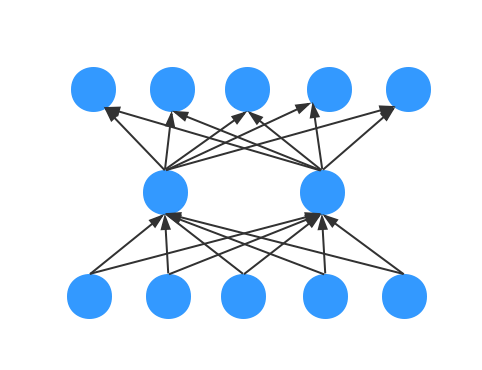
\includegraphics[width = 0.8\linewidth]{figure/autoencoder}
\caption{Autoencoder}
\label{fig:ae}
\end{figure}

However, only using the structure of autoencoder may not effectively model the text. If we set the input of autoencoder as the vectors of all terms in one document and try to generate the condensed features of the document, there will be so many parameters to optimize and the structure of the text is not utilized. In order to solve the problem, the structure of recursive autoencoder was proposed to model the hierarchical structure. Figure 2 shows the structure of recursive autoencoder.
\begin{figure}[ht]
\centering
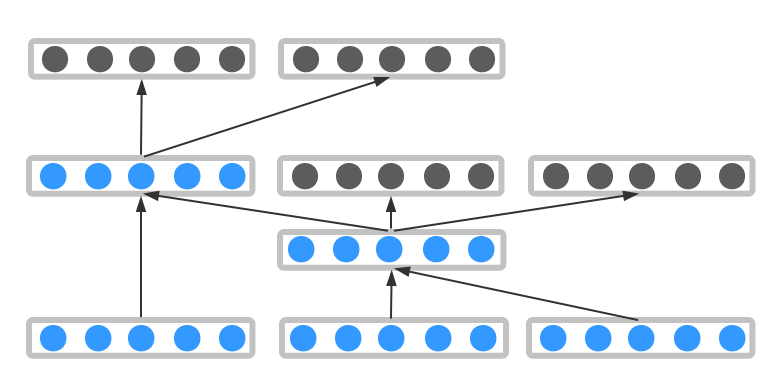
\includegraphics[width = 1.0\linewidth]{figure/recursiveautoencoder}
\caption{Recursive Autoencoder}
\label{fig:rae}
\end{figure}


In each layer, several terms are combined to generate the condensed features which will be utilized as the input of the next layer. At the final layer of recursive autoencoder, the vector of hidden layer will be the vector representation of the whole documents.

One of the key problem in such structure is how to combine different terms. There are mainly two ways. One way is to adopt the grammer tree which generated in advance. Each word will be combined in the same way as they are merge in the grammer tree. Another way is to utilize the greedy algorithm. At each layer, each pair of the adjacent words will be first combined and output reconstruction error. Then the pair of words with smallest error will be first combined. Using this greedy algorithm, the vector of each document can also be generated. In the experimental part, the effectiveness of the two structured will be compared.

\subsection{Semi-supervised Recursive Autoencoder}
In the traditional recursive autoencoder model, the network is trained only by the document itself. Therefore, it is the unsupervised model. In certain scenario, the label information of documents can be incorporated into the model and turn the model into a semi-supervised model.

One of the semi-superivised recursive autoencoder model has been proposed by socher et al.\cite{socher2011semi} in order to handle the issue of sentiment analysis. The structure of recursive autoencoder is presented as follows:
\begin{figure}[ht]
\centering
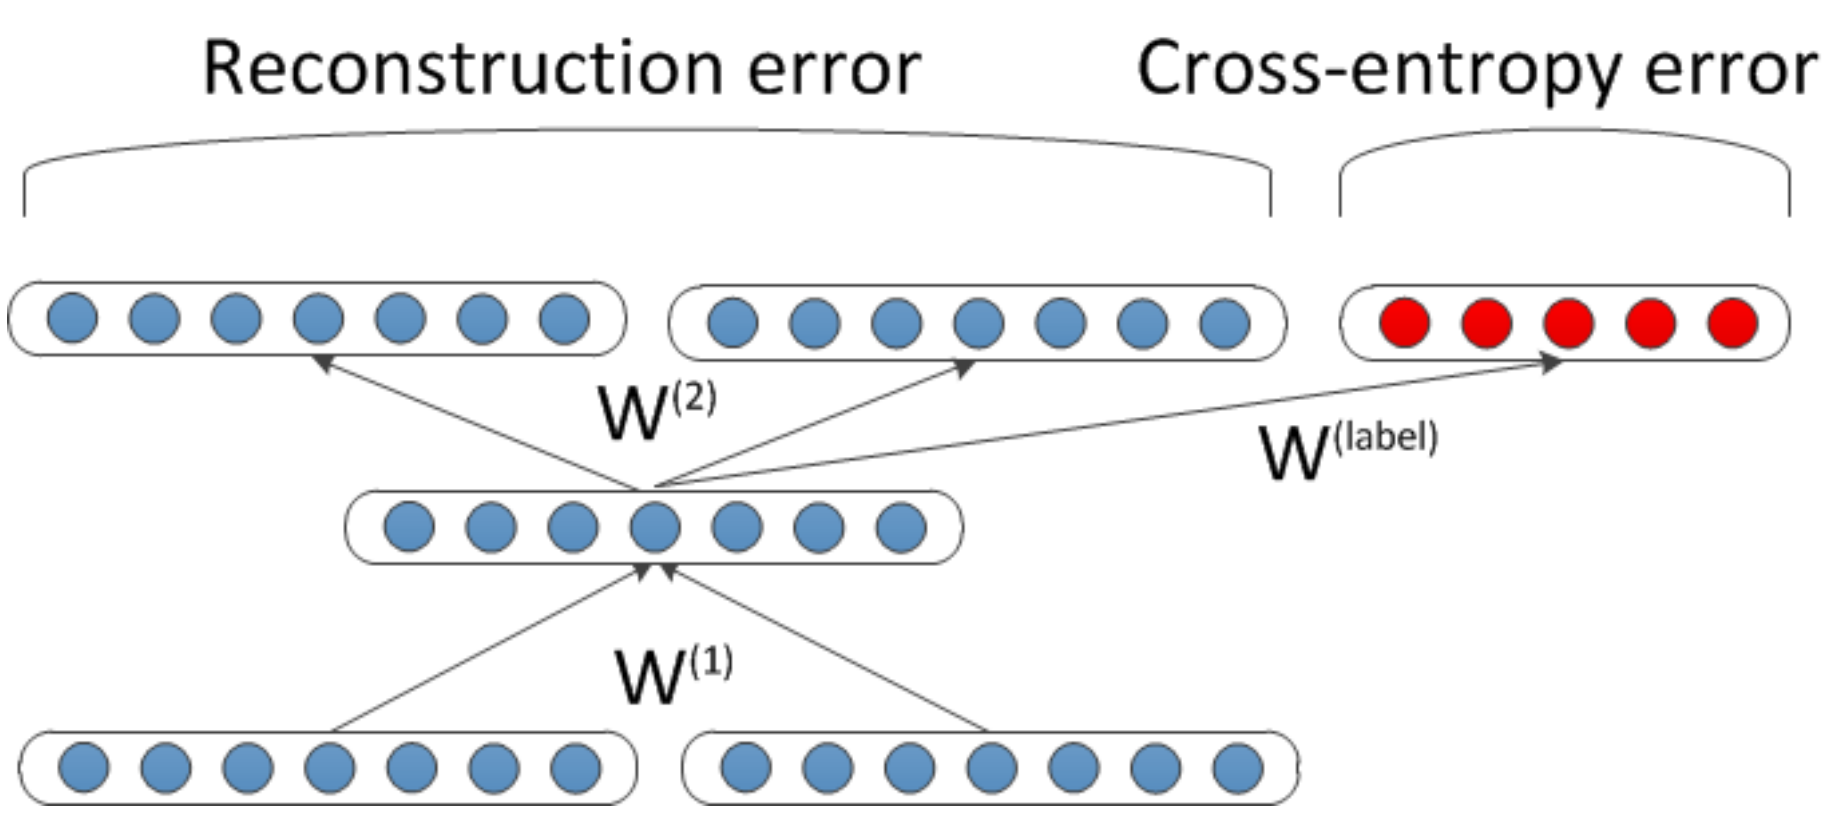
\includegraphics[width = 1.0\linewidth]{figure/semiautoencoder}
\caption{Semi-supervised Autoencoder}
\label{fig:sae}
\end{figure}	
	
As we can see from the figure, the input of the model is also the distributed representation. After being processed by the hidden layer, the output layer reconstructs the input vector. In order to measure the performance of the representation, the reconstruction error is computed as the distance between the input vector and output vector. Also we can assign different terms with different weights. So
\begin{equation}
\begin{split}
 & E_{rec}([c_{1};c_{2}];\theta) \\
 & = \frac{n_{1}}{n_{1}+n_{2}} ||c_{1}-c_{1}'||^2 + \frac{n_{2}}{n_{1}+n_{2}} ||c_{2}-c_{2}'||^2\\
 \end{split}
\end{equation}
, where n denote the number of words. In addition, c denotes the vector of input and c' present the vector of output.

Also, in order to predict the sentiment of the sentence, an extra output unit is added to generate the sentiment label. And this generated label will be compared with the correct label. A softmax function is utilized in this scenario to generate the probability of each label. And author use the cross-entropy error to measure the correctness of the model.
\begin{equation}
\begin{split}
 & E_{cE}(p,t;\theta) \\
 & = -\sum_{k=1}^{K}{t_{k}\log{}d_{k}(p;\theta)}\\
 \end{split}
\end{equation}
, where $t_{k}$ denotes the target label and $d_{k}$ denotes the probability of each label.

After combining the two process, we can compute the reconstruction error and cross-entropy error. And the objective is to minimize the weighted sum of the two errors as follows:
\begin{equation}
\begin{split}
 & E([c_{1}; c_{2}]s, ps, t, θ) = \\
 & = \alpha E_{rec}([c_{1}; c_{2}]_{s}; \theta) + (1 - \alpha)E_{cE}(p_{s}, t; \theta).
\\
 \end{split}
\end{equation}
	\section{Experiment and Results}
%    \begin{table}[h]
%        \begin{tabular}{|l|l|l|}
%            \hline
%            Model               & Precision & Recall \\ \hline
%            tf-idf              &           &        \\ \hline
%            Bayesian Classifier &           &        \\ \hline
%            Lexical Chain       &           &        \\ \hline
%            RNN                 &           &        \\ \hline
%            RNN-Word2Vec        &           &        \\ \hline
%        \end{tabular}
%    \end{table}
		\begin{figure}
			\centering
			\caption{Precision Comparison}
			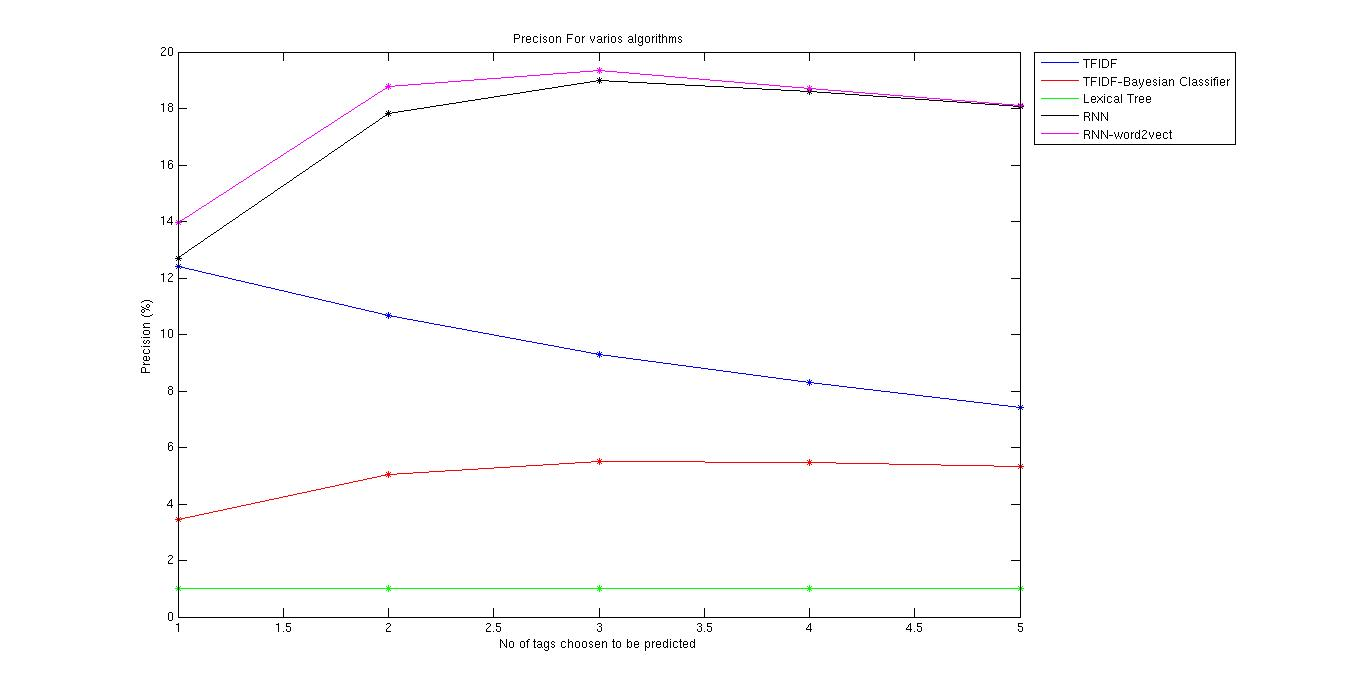
\includegraphics[scale=0.3]{../baseline/precision.jpg}
            \label{precision}
		\end{figure}
		\begin{figure}
			\centering
			\caption{Precision Comparison}
			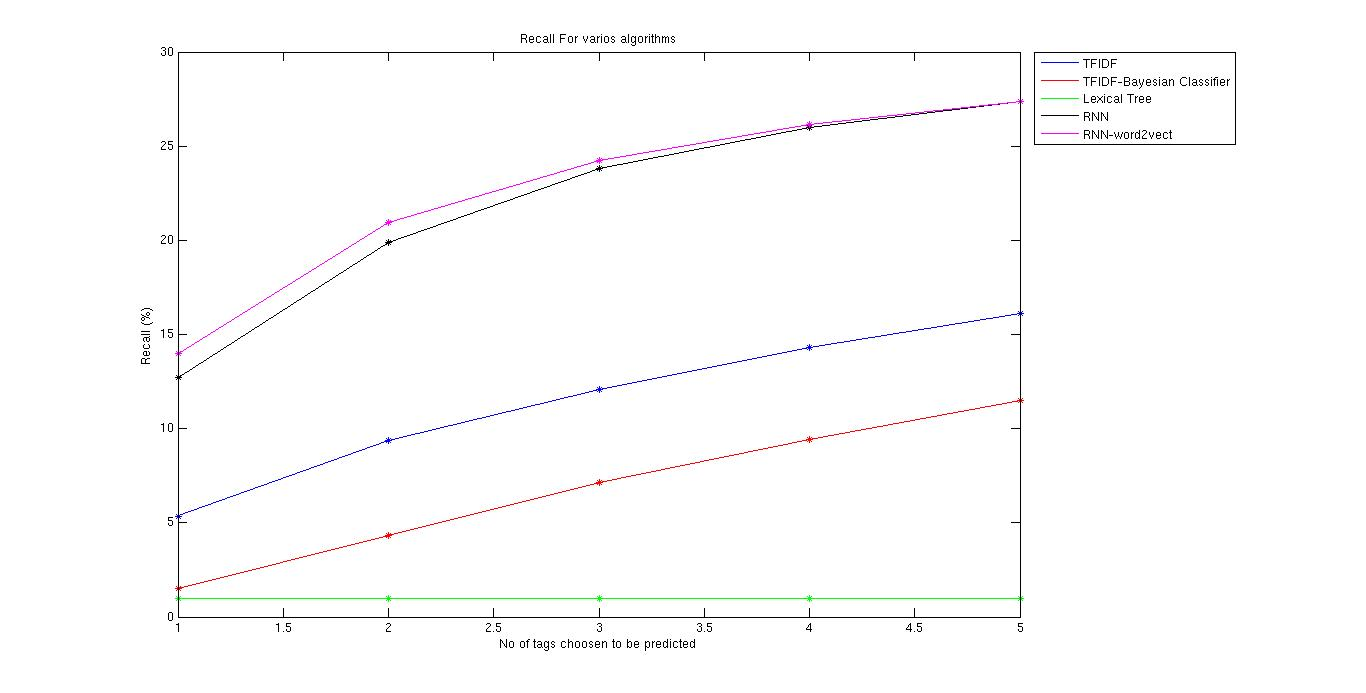
\includegraphics[scale=0.3]{../baseline/recall.jpg}
            \label{recall}
		\end{figure}
		\subsection{Baseline Algorithm Results}
		
		
		To evaluate the performance of our approach compared to existing techniques, we have used Precision and Recall rates as our benchmarking standards.
		We have formally defined these parameters as 
		
		$Precision = \frac{ sizeof(A \bigcap B)}{sizeof(A)}$
		
		$Recall    = \frac{ sizeof(A \bigcap B)}{sizeof(A)}$
		
		where A is the set of predicted tags and B is the set of actual tags.
		
		We have implemented TF-IDF and Bayesian Classifier approach as described by the survey for Keyword Extraction on our data set. With plain vanilla TF-IDF, the average precision and recall rates were less than 10 \%. However, after preprocessing the data by using a stemmer, the accuracy is a modest 15-20\% on topics in our data set for as the best performer.
		We have used portland stemmer, available as part of open source NLTK(Natural Language Processing Toolkit) project.
		The Bayesian Classifier is similar to TF-IDF approach except that it takes into account the position of the word in text. The weight of each term is reduced as the log of the its position from the beginning of the sentence.
		
				
		As part of survey paper\{cite\}, we found out that the existing standard for key word extraction uses Lexical Tree approach and hence we have summarized its performance on our data set as well. As per the lexical tree approach, the precision and recall were very poor, less than 1 \% when tested against our data set. The reason for this can be attributed to the fact that our documents are very small posts with about a paragraph in them. Siber and McCoy\cite{silber2002efficiently} had implemented this feature for larger documents such as conference papers , essays etc and they would have probably had a document with more than 25 nouns, contrary to this, we only had 4-8 nouns per document on an average, hence we could not build a bigger graph for our documents. 
		
		\subsection{Dataset}
		
		We had identified data from stackexchange( \url{https://archive.org/download/stackexchange/stackexchange_archive.torrent}) to be a suitable data set for our project. 
		`
		Of the 20 GB, available to us, for the feasibility of the experiment, we are using only 95 MB of data, which we have cleaned and formatted for our applications, on about 5 topics for our evaluation. Although the data set seems to be small compared with original one, we felt this was enough for testing purposes. Later we will try to \textbf{increase the data set} when our model is finished.
        
        Here is an interesting question, why we choose several topic and not only one topic as small data set to test our model? In fact we did that, but found that it's not a good way to do testing of the task like keyword extraction. For a single topic, some words will occur frequently, for example, in the topic of \emph{apple}, the words like \emph{osx} and \emph{iphone} will occur frequently in most documents which according to \emph{tf-idf}, they are not important words. But in fact they are the tags for many documents in this topic. And if we train the model on only a single dataset, then if the model only predict the top frequently tags, it can still gain good performance. That's the reason we use several topics as dataset here.
        
        The last step is to dived the data set into training dataset and testing dataset. I random sample 20\% as the testing dataset and the rest are the training dataset. The number of documents in each data set is: 37935 for testing data set and 152537 for training data set.
        \subsection{Our Model}
        Our work is based on the open source software \footnote{https://github.com/sancha/jrae}. For the midterm report, we use the tool to do some simple checking and we also modify some parts of the it to make use of the word vectors generated by \emph{word2vec}\footnote{https://code.google.com/p/word2vec/}, another tool developed by Google.
        
         \begin{figure}
         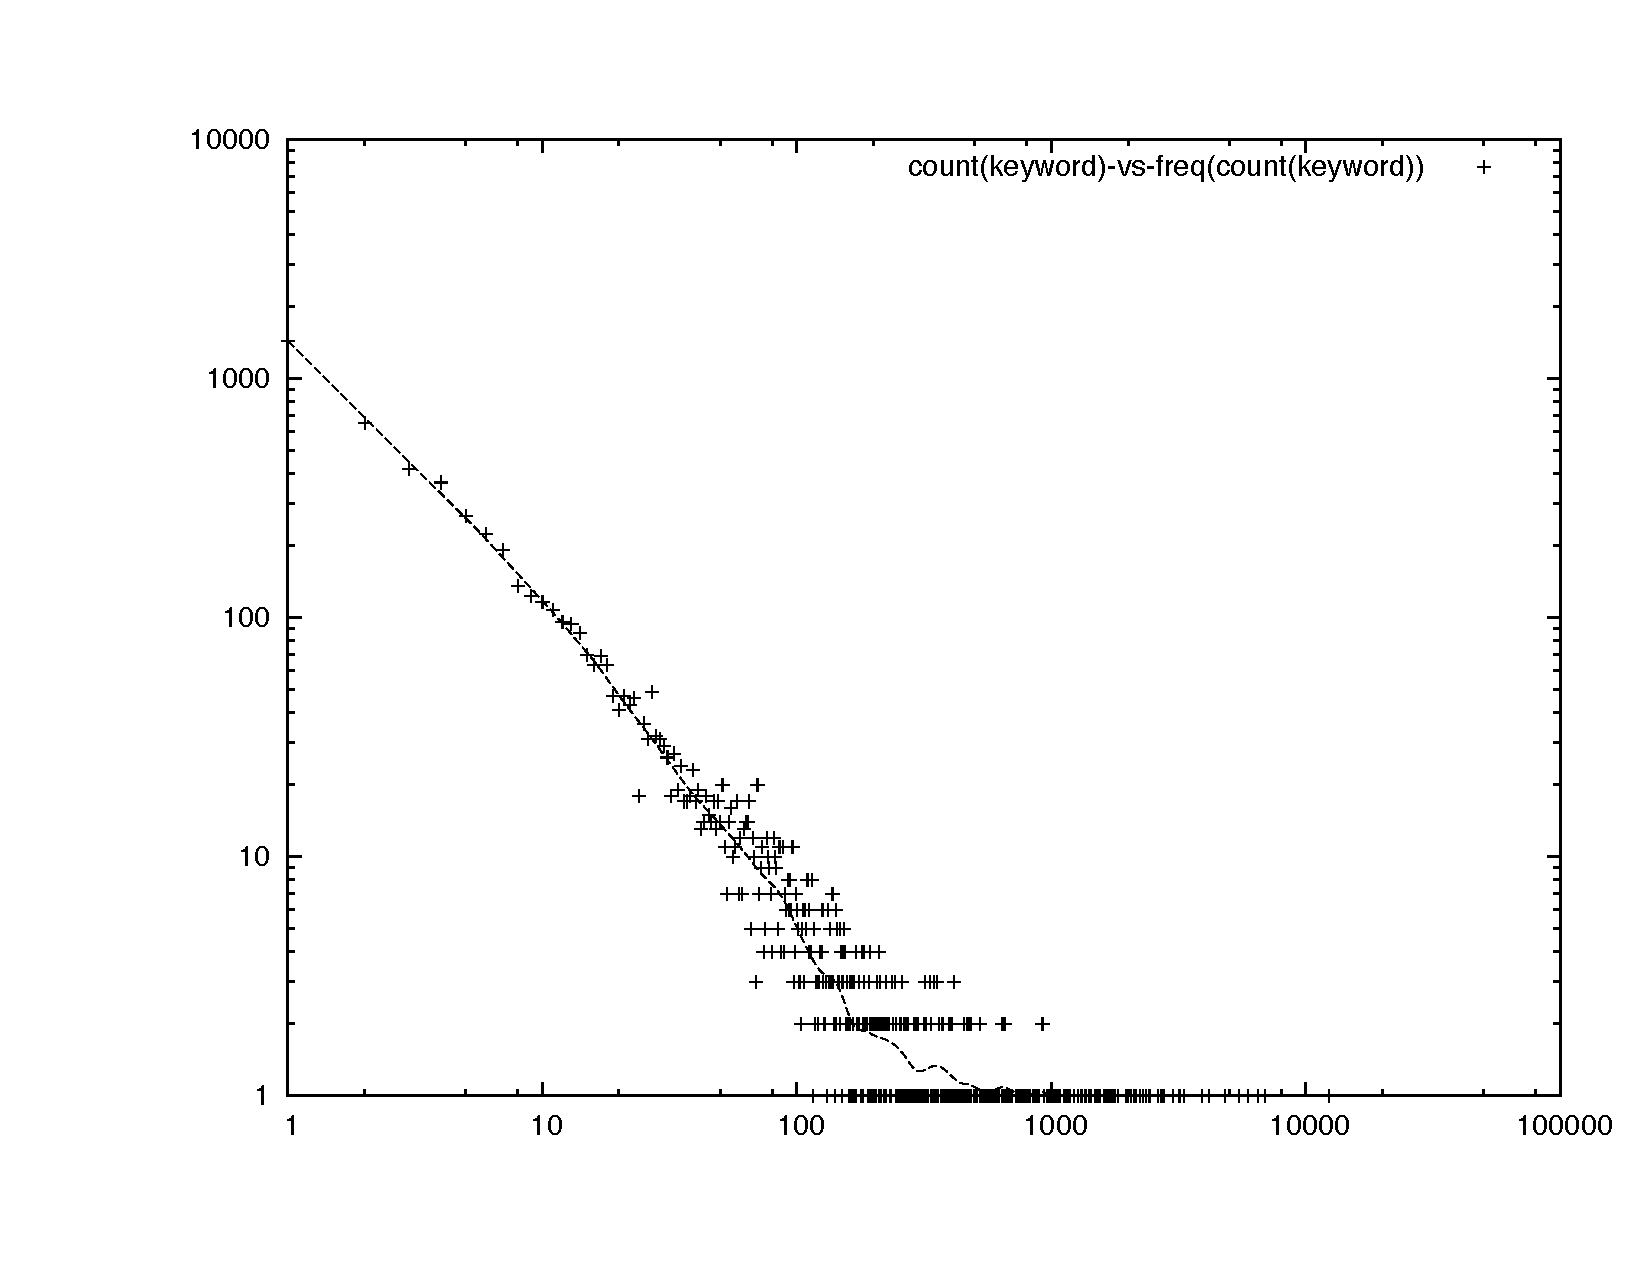
\includegraphics[scale=0.5]{dist.pdf}
         \caption{The distribution of tags follows Zipf's law. Here the x-axis is the count of the tag and the y-axis is the frequency of the count of tags. Drawn in log-log scale.}
         \label{zips}
        \end{figure}
        
        Before discussing about the experiment, we will introduce the method about training data preprocessing. We analyze the distribution of the tags in the dataset, and we find it follow Zipf's law from Figure \ref{zips}. So we can't train the model with all dataset. And here, our model is a supervised model, and it's a multi-class classification task so it's better not to train the model on all the labels. Here, we just choose the top 200 big tags and for each tag we sample 100 documents.
        
        Besides, our task is a little different with the classical classification task. For each document, we may give more than one tag, because it's common for a document having more than one tag. So when predicating, we generate the belief of each tag for each document and choose the top-n tags.
        
        We do the testing on these settings:\begin{inparaenum}[(i)]
            \item original model
            \item pre-training the parameters of word vectors.
        \end{inparaenum}. We trained the model with 10 dimension word vector.
        
        From the Figure \ref{precision} and \ref{recall} above we see the difference between the two models are less and less with the increasing of the number of tag returned. It's because that the tag pool is only 200. In fact if we don't do filtering of the tags, our model achieves 3.9\% for precision and 8.7\% for recall, while the original model achieves only 1.4\% for precision and 3.1\% for recall, which means our model rank the right tags higher than the original one.
        
        We see the precision and recall rate is not so high. Some reason for it is because we only train on the top-200 high frequent tags. And the ratio of them in the testing data is 49595/85108. It means that we can only achieve the recall rate with 58\% at most.
	\section{Pending Work}
    \begin{figure}
        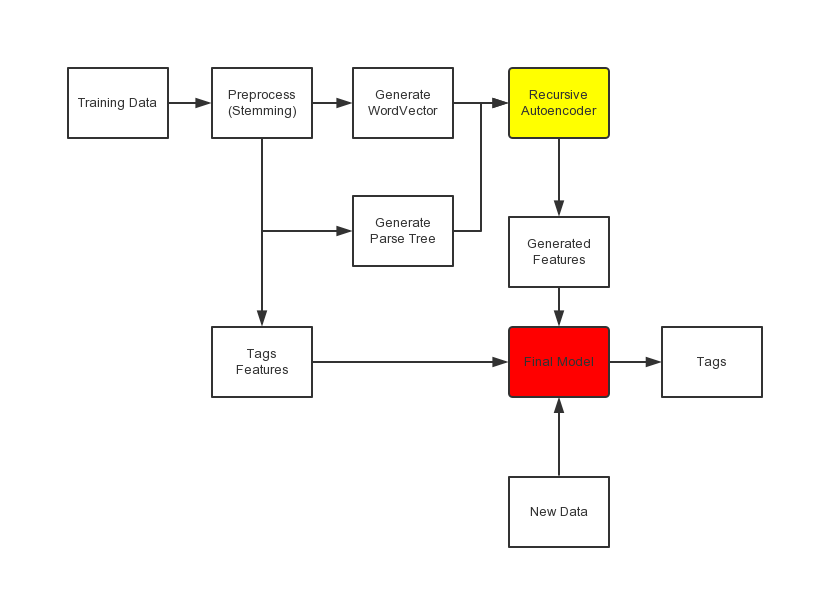
\includegraphics[scale=0.6]{DataFlow.png}
        \caption{Our frame for keyword extraction. Here we have done some work on the yellow part: Recursive Autoencoder.}
        \label{frame}
    \end{figure}
    Now we have studied and implemented some baseline algorithms. We also the recursive autoencoder algorithm mentioned in the proposal. What's more we have done some experiment based on recursive autoencoder and also integrate \emph{word2vect} with recursive autoencoder.
    
    In Figure \ref{frame} is our big frame for the task. For the final report, we will add parse tree into the recursive autoencoder instead of using the greedy algorithm.
    
    And for the final model:\textbf{TODO}
    
    What's more we will also try to increase the size of the word vectors and the number of training data to observe the performance of our model.
    
    Besides, we have to admit if not filtering the tags not in the target documents, the result is worse since here in our dataset, for most tags they appear in the documents. Now we just use a simple to use this information, later we will try to train our model with this information.
	\bibliography{bib/dp}
	\bibliographystyle{plain}


\end{document}